% METODOLOGÍA

\cleardoublepage

\chapter{Metodología y Desarrollo}
\label{chapter-metodologia-desarrollo}

La idea general del \textit{transfer learning} es preentrenar un modelo usando una red neuronal de gran tamaño sobre un dataset de gran volumen para después ajustar la red (\textit{fine-tunning}) usando un dataset mucho más reducido y ajustado a la tarea especifica que se intenta resolver. El aprendizaje por transferencia marca una gran diferencia y nos permite resolver nuevos problemas mucho más fácilmente, ya que normalmente podemos cargar pesos previamente entrenados de un modelo sin requerir de un gran conjunto de datos para resolver una tarea específica.

BERT es un modelo de lenguaje preentrenado que ha demostrado que el concepto de la transferencia del aprendizaje ha resultado ser una herramienta poderosa no solo en los problemas de visión por computacdora (\gls{gls_computer_vision}, en inglés), sino también en el procesamiento natural del lenguaje y que podría ser suficiente con un ligero ajuste (\textit{fine-tunning}) implementar un nuevo modelo que resuelva de forma satisfactoria  una nueva tarea.

El \textit{transfer learning} se convirtió en la estrategia predeterminada en la visión por computadora alrededor del año 2014. A menudo usaban modelos que estaban entrenados previamente para la clasificación de imágenes en Imagenet \cite{Olga2015Imagenet}, lo que significaba que usaban aprendizaje supervisado y un gran conjunto de datos con etiquetas para entrenar previamente el modelo. Durante varios años se estuvo investigando sin éxito formas de usar el aprendizaje por transferencia en el procesamiento del lenguaje natural y se estuvo tratando de encontrar tareas y conjuntos de datos con las mismas propiedades atractivas que tenía Imagenet para la visión por computadora. Finalmente, en 2018 al menos tres artículos diferentes (BERT \cite{https://doi.org/10.48550/arxiv.1810.04805}, ELMo \cite{Peters2018Elmo}, GPT \cite{radford2018improving}) demostraron que se puede usar el \textit{transfer learning} también en el procesamiento natural del lenguaje. 

Entre estos modelos, se puede decir que BERT fue el más limpio, ya que requirió la menor cantidad de \textit{fine-tunning}, un conjunto de datos más pequeño y, en general, también dio los mejores resultados.

Basados en estos conceptos de \textit{transfer learning} y \textit{fine-tunning} procederemos a evaluar el uso y el desempeño de BERT en la resolución de problemas de procesamiento natural del lenguaje siguiendo los siguientes pasos:

\begin{enumerate}
  \item \textbf{Selección de problemas} \\
  En esta primera etapa elegimos un par de problemas típicos del procesamiento natural del lenguaje pero que a su vez sean distintos a los problemas para los que BERT fue entrenado inicialmente. La idea es poder demostrar la adaptabilidad del modelo para resolver cualquier clase de problemas basado en la arquitectura propia de BERT. Los problemas con los que trabajaremos son el Análisis de Sentimiento (clasificación) y la tarea de Respuesta a Preguntas.
  \item \textbf{Selección de los conjuntos de datos (\textit{datasets})} \\
  En cuanto a la selección de los \textit{datasets} se decidió trabajar con conjuntos de datos asociados a cada uno de los problemas antes descritos, procurando que los \textit{datasets} elegidos permitan establecer indicadores de comparación y que existan estudios de comparación del desempeño con otros modelos y soluciones. Para el caso de análisis de sentimiento se trabajará con un \textit{dataset} de reseñas de películas de IMDB creado por investigadores de la Universidad de Stanford, para el problema de preguntas y respuestas se trabajó con el conocido \textit{dataset} SQuAD en su versión 1.0.
  \item \textbf{Fine Tuning de BERT} \\
  Para cada uno de los problemas elegidos se hizo un ajuste del modelo inicial de BERT usando para el entrenamiento un \textit{dataset} etiquetado. La intención es hacer las adecuaciones necesarias al modelo para intentar encontrar una solución simple a cada uno de los problemas elegidos.
  \item \textbf{Evaluación de los resultados} \\
  Se compararon los resultados obtenidos en cada problema con otros modelos implementados para resolver el problema. La idea es validar que simplemente haciendo un pequeño \textit{fine-tunning} del modelo original podemos obtener resultados similares o cercanos a los del estado del arte en cada problema.
\end{enumerate}

\clearpage 
%%%%%%%%%%%%%%%%%%%%%%%%%%%%%%%%%%%%%
% SECTION - ANÁLISIS DE SENTIMIENTO 
%%%%%%%%%%%%%%%%%%%%%%%%%%%%%%%%%%%%%

\section{Problema de Análisis de Sentimiento (Clasificación)}
\label{section-analisis-de-sentimiento}

%%%%%%%%%%%%%%%%%%%%%%%%%%%%%%%%%%%%%%%%%%%%%%%%%%%%%%%%%%%%%%%%%%%%%%%%%%%%%%%%%%%%%%%%%%%%%%%%%%%%%%%%%%%%%%%

\subsection{Descripción del problema}
\label{subsection-as-descripcion-problema}

El análisis de sentimiento es un subcampo del procesamiento de lenguaje natural que ha tenido un gran desarrollo en los últimos años. Este interés ha sido alimentado en gran parte por el auge de las redes sociales que ha dado lugar a la aparición de blogs, foros y aplicaciones en línea que le permiten a los usuarios discutir sobre cualquier tema y compartir sus opiniones. Este tipo de análisis es ampliamente usado por distintas empresas para entender la opinión de sus clientes y conocer la aceptación de sus productos y servicios. 

A través del análisis de sentimiento las empresas pueden estudiar los comentarios de los clientes para prestar una mejor atención, crear mejores productos o mejorar sus estrategias de marketing para atraer nuevos clientes. En líneas generales los resultados del análisis de sentimiento ayudan a conocer mejor los intereses y opiniones de los clientes sobre las tendencias del mercado.

El objetivo principal del problema es analizar una secuencia de texto y a partir de ella identificar o extraer información subjetiva que permita inferir si el sentimiento asociado a la frase es positivo o negativo. Desde otro punto de vista, se trata de una tarea de clasificación de la polaridad asociada a los textos que pueden estar presentes en documentos, oraciones u opiniones de forma masiva y automática. 

En el estudio de \cite{Bhavitha_sa}, los autores señalan que las técnicas de análisis de sentimientos se pueden clasificar en tres enfoques distintos en cuanto a la forma de solución.
\begin{enumerate}
  \item \textbf{Enfoque de aprendizaje automático:} Cuando utilizamos modelos de \textit{machine learning} en la solución del problema y generalmente nos basamos en un modelo especifico a partir del entrenamiento sobre un gran corpus de documentos.
  \item \textbf{Enfoque basados en léxico:} Mediante este enfoque, la orientación semántica de las palabras de un texto se calcula obteniendo las polaridades de las palabras a partir de un léxico predefinido. Es decir, habrá palabras en el texto que por si sola denotan ya una polaridad. Ejemplo, palabras como \textit{magnifico, bueno, grandioso, espectacular}, tienen un sentido positivo, mientras que palabras como \textit{horrible, malo, decepción}, tienen un significado negativo.
  \item \textbf{Enfoque híbrido:} Se basa en la combinación de información lingüística y estadística, reglas semánticas junto con el uso de redes neuronales profundas.
\end{enumerate}

Más recientemente, se utilizan técnicas de aprendizaje profundo, como BERT, T5 y GPT, para entrenar clasificadores de sentimientos de alto rendimiento que se evalúan mediante métricas como F1, recuperación y precisión. 

%%%%%%%%%%%%%%%%%%%%%%%%%%%%%%%%%%%%%%%%%%%%%%%%%%%%%%%%%%%%%%%%%%%%%%%%%%%%%%%%%%%%%%%%%%%%%%%%%%%%%%%%%%%%%%%

\subsection{Selección del Dataset}
\label{subsection-as-dataset-imdb}

Para evaluar los sistemas de análisis de sentimientos, se utilizan generalmente conjuntos de datos de referencia como:

\begin{itemize}
    \item \textbf{SST (Stanford Sentiment Treebank):} es un corpus con árboles de análisis sintáctico completamente etiquetados que permite un análisis completo de los efectos compositivos del sentimiento en el lenguaje. El corpus se basa en el conjunto de datos presentado por \citep{PANG_LEE_SST_https://doi.org/10.48550/arxiv.cs/0506075} y consta de 11.855 oraciones individuales extraídas de reseñas de películas. Se analizó con el analizador de Stanford e incluye un total de 215154 frases únicas de esos árboles de análisis, cada una anotada por 3 jueces humanos.
    Cada frase está etiquetada como negativa, algo negativa, neutral, algo positiva o positiva. El corpus con las 5 etiquetas se denomina SST-5 o SST de grano fino. Los experimentos de clasificación binaria en oraciones completas (negativas o algo negativas versus algo positivas o positivas con oraciones neutras descartadas) se refieren al conjunto de datos como SST-2 o SST binario.
    
     \item \textbf{GLUE (General Language Understanding Evaluation benchmark):} es una colección de nueve tareas de comprensión del lenguaje natural, que incluyen tareas de una sola oración CoLA y SST-2, tareas de similitud y paráfrasis MRPC, STS-B y QQP, y tareas de inferencia del lenguaje natural MNLI, QNLI, RTE y WNLI.
     
     \item \textbf{Large Movie Review Dataset IMDB:} es el conjunto de datos que se seleccionó para este experimento y que se procederá a describir a continuación.
\end{itemize}

El \textit{\textbf{Large Movie Review Dataset IMDB}} es un conjunto de datos con 50.000 reseñas de películas creado para la clasificación de sentimientos binarios que contiene sustancialmente más datos que los otros conjuntos de datos de referencia.

Como describen los creadores de este \textit{dataset} en su \textit{paper} del 2019 \textit{Learning Word Vectors for Sentiment Analysis} \cite{maas-EtAl:2011:ACL-HLT2011}, este conjunto de datos fue creado a partir de reseñas de películas realizadas por la audiencia y extraídas del sitio público IMDB. Para la construcción del mismo consideraron no incluir más de 30 reseñas por película.

Este conjunto de datos se encuentra balanceado, es decir, contiene un mismo número de reseñas positivas y negativas. Los autores para construirlo consideraron solo críticas altamente polarizadas en base al sistema de rating que tiene IMDB y de esa forma consideraron una crítica negativa a aquellas reseñan que tenían una puntuación $\leq$ 4 sobre 10 y positiva si la puntuación era $\geq$ 7 sobre 10. Las reseñas neutrales no fueron incluidas

Para el propósito de este trabajo se usó una versión del \textit{dataset} original transformado y disponible en la plataforma \textit{kaggle.com} \citep{n_2019}. Esta versión ha sido transformada a un archivo de valores separados por comas, CSV (del inglés comma-separated values), en el cual se presentan dos columnas una para la reseña y otra para el sentimiento.

La razón por la que se escogió este \textit{dataset} y no otro es la amplia cantidad de soluciones desarrolladas tomando como base de entrenamiento el mismo, esto permitirá poder hacer un estudio del resultado obtenido y compararlo con otros modelos.

%%%%%%%%%%%%%%%%%%%%%%%%%%%%%%%%%%%%%%%%%%%%%%%%%%%%%%%%%%%%%%%%%%%%%%%%%%%%%%%%%%%%%%%%%%%%%%%%%%%%%%%%%%%%%%%

\subsection{Estado del arte}
\label{subsection-as-estado-del-arte}

Para evaluar el estado del arte relacionado a la solución de análisis de sentimiento sobre el \textit{dataset} de reseñas de IMDB se utilizaron diversas fuentes. 

En el trabajo de \cite{Dang_2020} los autores analizaron y realizaron una comparación entre distintos estudios que usan el aprendizaje profundo como las \acrlong{acr_dnn} (\acrshort{acr_dnn}, por sus siglas en inglés), \acrlong{acr_rnn} (\acrshort{acr_rnn}, por sus siglas en inglés) y \acrlong{acr_cnn} (\acrshort{acr_cnn}, por sus siglas en inglés), para resolver diferentes problemas asociados al análisis de sentimiento. En este estudio no se incluyeron las recién aparecidas (para ese momento) redes basadas en Transformers. Los autores usaron distintos datasets para la evaluación entre ellos el mismo utilizado en este trabajo \ref{subsection-as-dataset-imdb} y utilizaron en el preprocesamiento de los datos dos técnicas distintas de procesamiento de texto (\gls{gls_wordembeddings} y \gls{gls_tfidf}). En sus conclusiones, los autores deducen una fiabilidad ligeramente superior en la mayoría de conjunto de datos con las redes neuronales recurrentes, sin embargo, igual mencionan un tiempo de cálculo mucho más largo, como se puede evidenciar en las imágenes \ref{fig-as-eda-accuracy-comparison} y \ref{fig-as-eda-cpu-comparison} 

\begin{figure}[ht!]
    \centering
    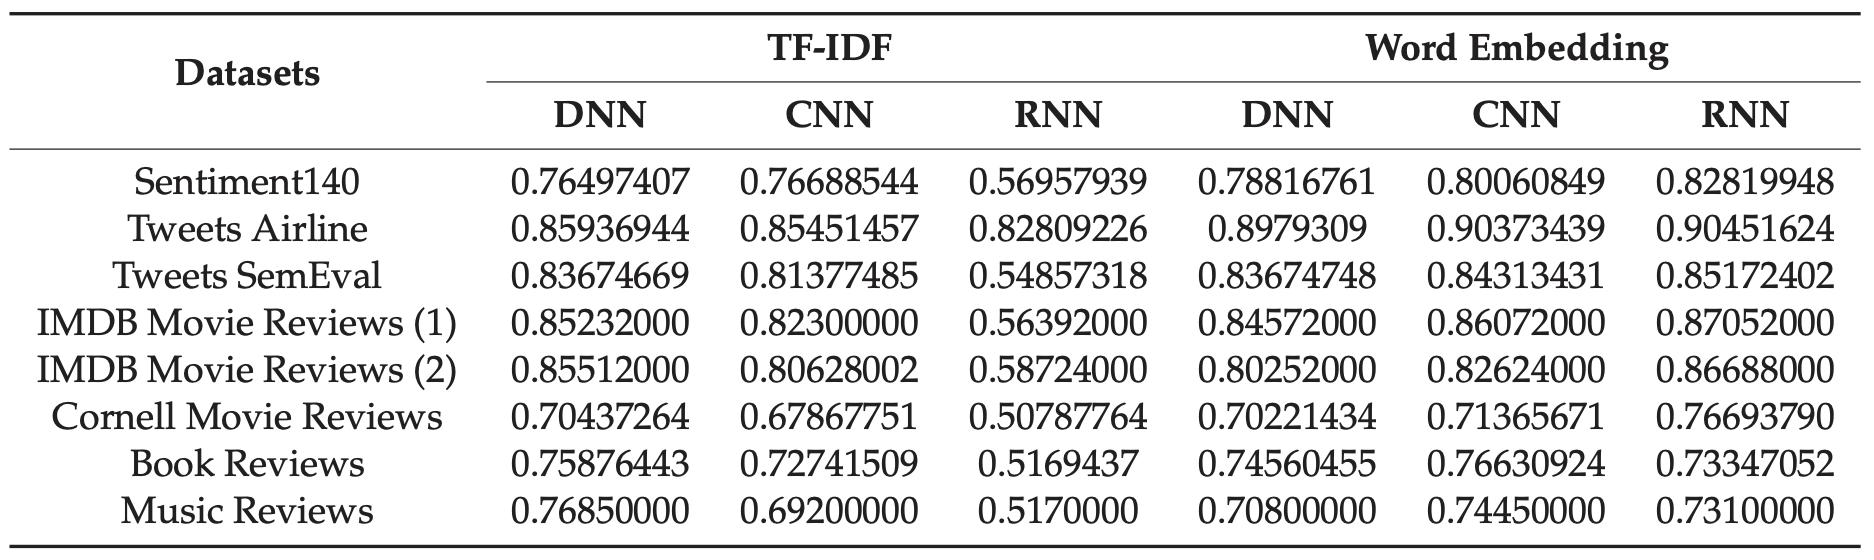
\includegraphics[scale=0.45]{figuras/as-eda-accuracy-comparison.png}
    % \caption[Así aparece el rótulo en el índice]{Así aparece el rótulo en el texto.}
    \caption[Análisis de Sentimiento - Tabla - Accuracy]{Comparación del accuracy obtenido para datasets con dos clases (positivo y negativo), en el artículo \textit{Sentiment Analysis Based on Deep Learning: A Comparative Study}. \textbf{Fuente: \cite{Dang_2020}}}
    \label{fig-as-eda-accuracy-comparison}
\end{figure}

\begin{figure}[ht!]
    \centering
    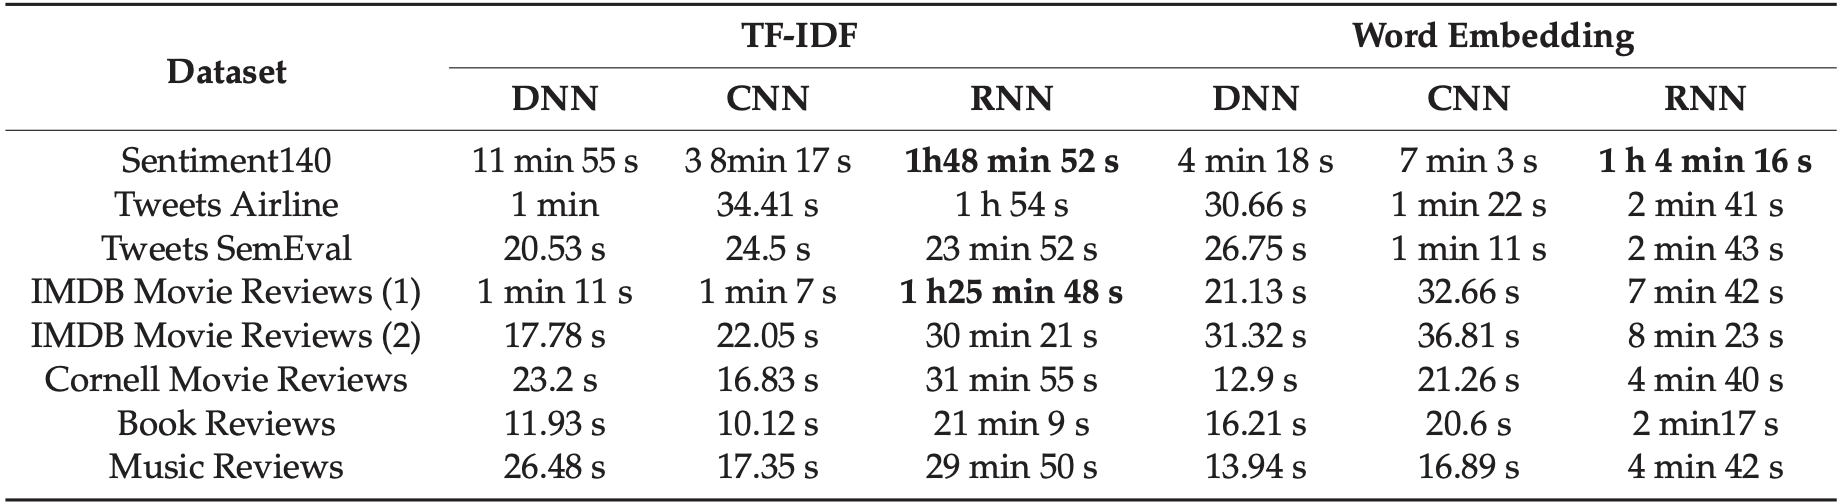
\includegraphics[scale=0.45]{figuras/as-eda-cpu-comparison.png}
    % \caption[Así aparece el rótulo en el índice]{Así aparece el rótulo en el texto.}
    \caption[Análisis de Sentimiento - Tabla - Performance]{\textbf{Comparación de los tiempos de cómputo experimentados para el entrenamiento de modelos con \acrshort{acr_gpu}, en el artículo \textit{Sentiment Analysis Based on Deep Learning: A Comparative Study}. Fuente: \cite{Dang_2020}}}
    \label{fig-as-eda-cpu-comparison}
\end{figure}

Es importante mencionar con respecto a este estudio que si bien las RNN evidenciaron tener un mejor desempeño con todos los datasets esto solo ocurrió con el uso de Word Embedding como técnica de preprocesado de los datos y no con \gls{gls_tfidf}.

Adicionalmente nos basamos en el sitio web NLP-progress (\url{https://nlpprogress.com/}) \cite{Ruder_NLP-progress_2022}, el cual es un repositorio en linea que hace un seguimiento del progreso en distintos problemas en el procesamiento del lenguaje natural NLP, incluidos los datasets y el estado del arte actual para las tareas de NLP más comunes.

Este repositorio muestra un ranking de modelos \ref{tbl-nlpprogress-ranking} que resuelven el problema de análisis de sentimiento haciendo uso del dataset de IMDB \ref{subsection-as-dataset-imdb}. En este ranking dos de los primeros tres modelos están basados en una implementación de BERT descrita por  \cite{FTBERTCLAS_https://doi.org/10.48550/arxiv.1905.05583} en su \textit{paper} ``\textit{How to Fine-Tune BERT for Text Classification?}'', y el modelo que presenta el mejor performance, XLNet \cite{XLNET_https://doi.org/10.48550/arxiv.1906.08237} es un método de preentrenamiento autorregresivo generalizado similar a BERT que permite aprender contextos bidireccionales mediante la maximización de la probabilidad esperada de todas las permutaciones del orden de factorización.

\begin{table}[ht!]
\resizebox{\textwidth}{!}{
\begin{tabular}{l|c|l}
\toprule
\textbf{Modelo} & \textbf{Accuracy} & \textbf{Paper} \\ \midrule
XLNet \cite{XLNET_https://doi.org/10.48550/arxiv.1906.08237}                    & 96.21     & XLNet: Generalized Autoregressive Pretraining for Language Understanding  \\ \midrule
BERT\_large+ITPT \cite{FTBERTCLAS_https://doi.org/10.48550/arxiv.1905.05583}    & 95.79     & How to Fine-Tune BERT for Text Classification?                            \\ \midrule
BERT\_base+ITPT  \cite{FTBERTCLAS_https://doi.org/10.48550/arxiv.1905.05583}    & 95.63     & How to Fine-Tune BERT for Text Classification?                            \\ \bottomrule
\end{tabular}
}
% \caption[Así aparece el rótulo en el índice]{Así aparece el rótulo en el texto.}
\caption[Análisis de Sentimiento - Ranking de modelos según NLPProgress]{\textbf{Ranking de modelos según NLPProgress (\url{http://nlpprogress.com/english/sentiment_analysis.html}) en la resolución de la tarea de análisis de sentimiento. Fuente NLPProgress}}
\label{tbl-nlpprogress-ranking}
\end{table}

Y por último citamos el ranking de otro reconocido sitio web \textit{Papers with Code} (\url{https://paperswithcode.com/}), el cual es un recurso de referencia para \textit{papers} científicos que representan el más actual estado del arte en distintas casuísticas del \textit{machine learning}. La plataforma está compuesta de casi 5.000 benchmarks, 2.300 tareas y 50.000 \textit{papers} que permiten comparar distintos enfoques en la resolución de distintos problemas.

Particularmente para el análisis de sentimiento sobre el dataset de IMDB, la plataforma compara distintas investigaciones rankeadas según el accuracy obtenido con este conjunto de datos. Es interesante observar que entre las 10 mejores soluciones encontramos 7 trabajos basados en Transformers y la mitad de ellos son modelos basados en BERT. (ver figura \ref{fig-as-eda-pwc-table})

\begin{figure}[ht!]
    \centering
    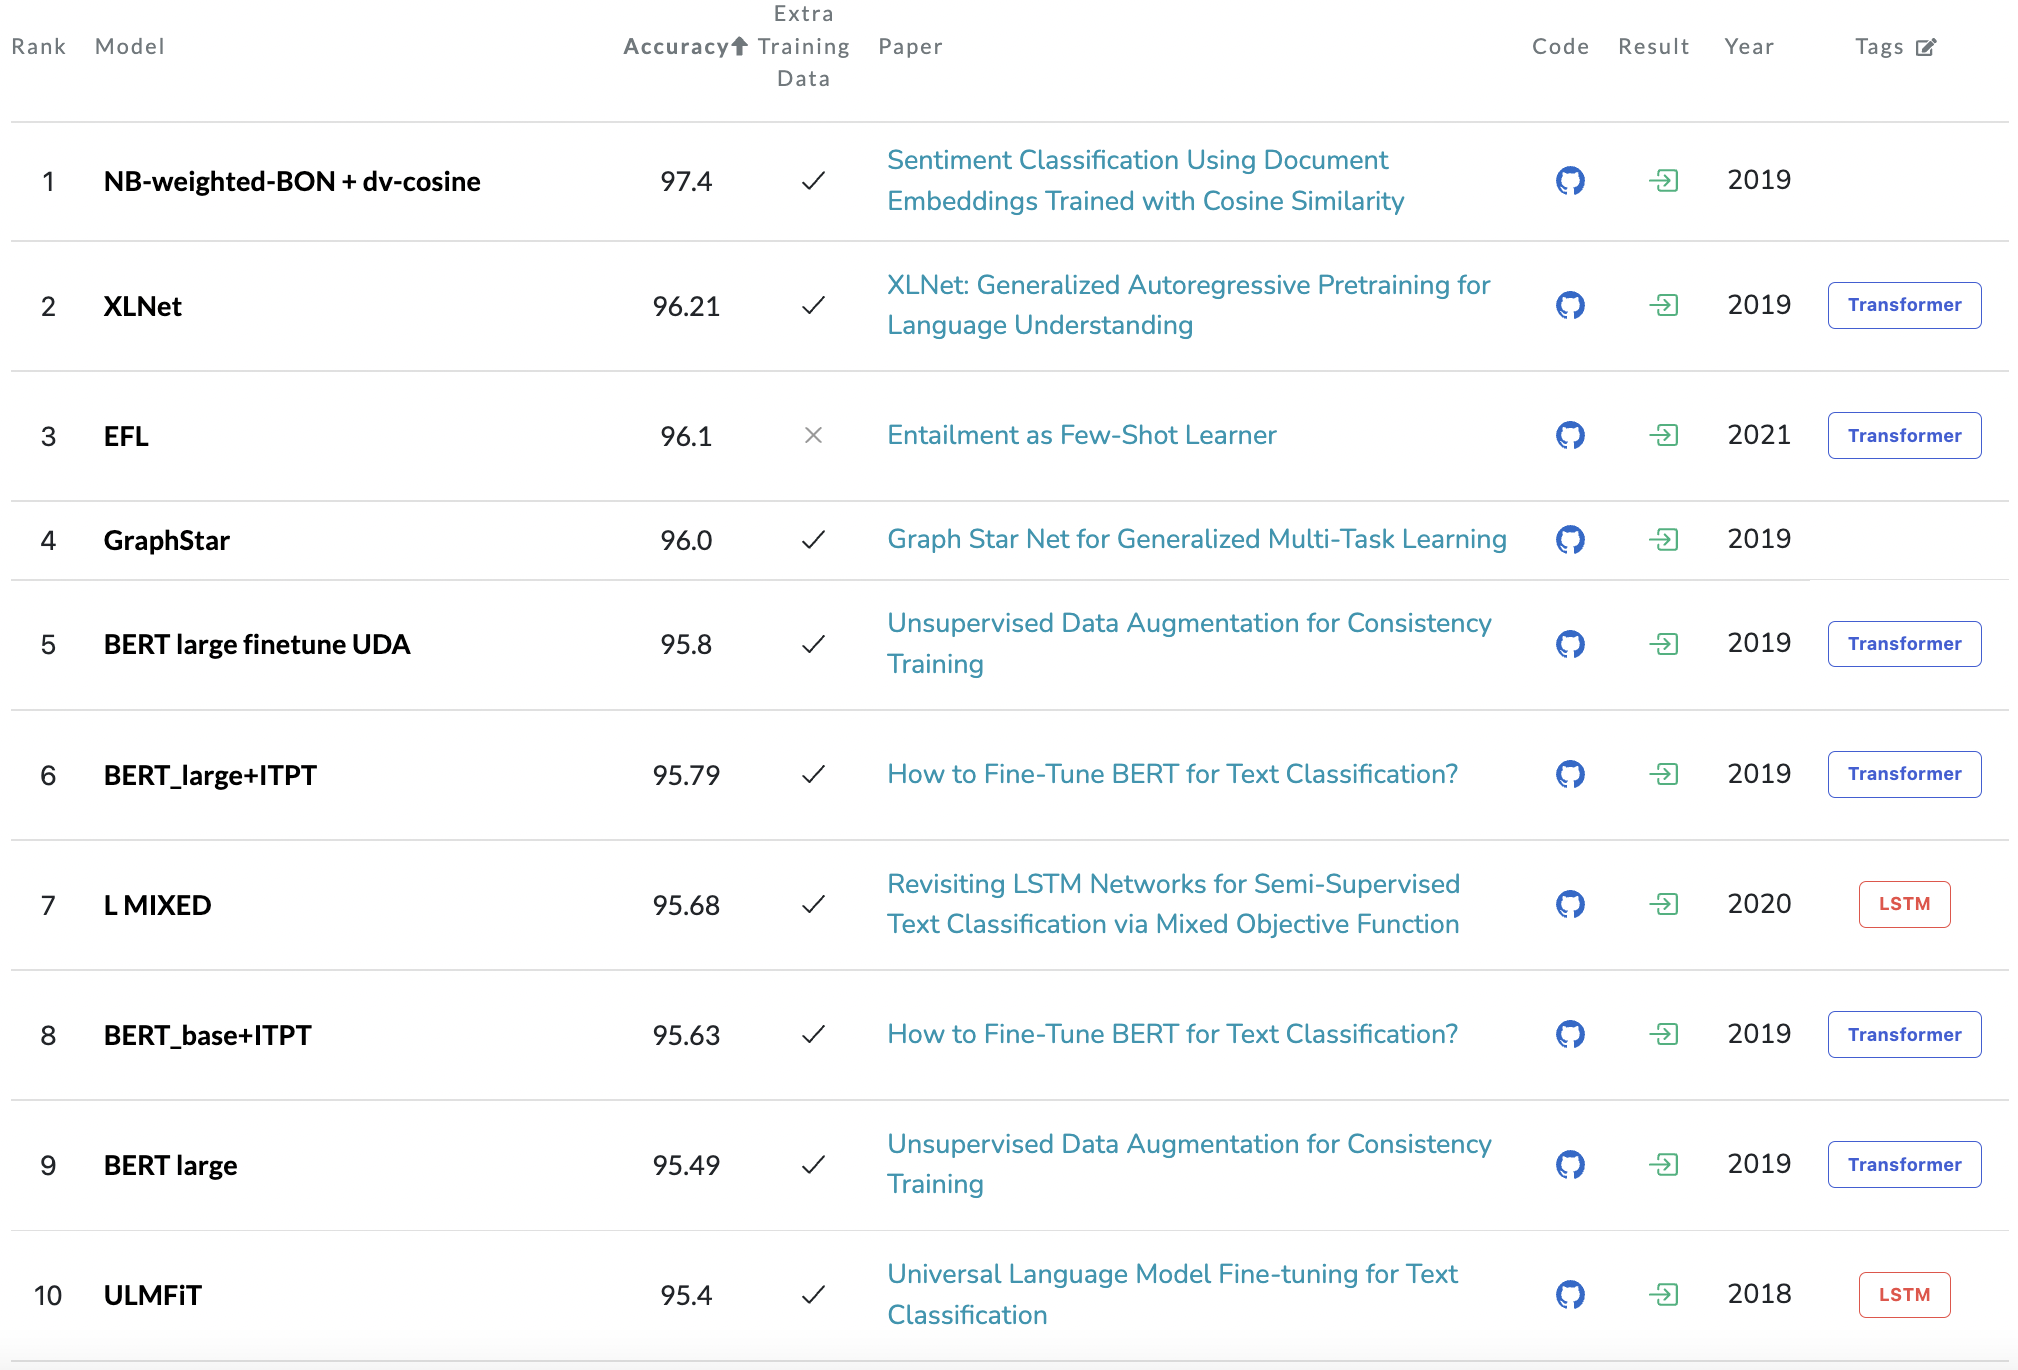
\includegraphics[scale=0.4]{figuras/as-eda-pwc-table.png}
    % \caption[Así aparece el rótulo en el índice]{Así aparece el rótulo en el texto.}
    \caption[Análisis de Sentimiento - Papers with code - Top 10]{\textbf{Esta imagen muestra el ranking de modelos organizados por el accuracy obtenido en el problema de análisis de sentimiento sobre el dataset de reseñas de IMDB. En este ranking podemos ver 7 modelos basados en transformers y la mitad de los modelos en el top 10 son modelos basados en BERT. Fuente: \url{https://paperswithcode.com/sota/sentiment-analysis-on-imdb}}}
    \label{fig-as-eda-pwc-table}
\end{figure}

%%%%%%%%%%%%%%%%%%%%%%%%%%%%%%%%%%%%%%%%%%%%%%%%%%%%%%%%%%%%%%%%%%%%%%%%%%%%%%%%%%%%%%%%%%%%%%%%%%%%%%%%%%%%%%%

\subsection{Arquitectura de la solución}
\label{subsection-as-arquitectura-de-la-solucion}
Como se mencionó anteriormente en la sección \ref{subsection-arquitectura-bert}, la arquitectura de BERT ha sido diseñada para adaptarse a la resolución de distintos problemas a través de un leve ajuste. Este caso en particular se trata de un problema de clasificación de una frase en dos clases objetivos, en otras palabras, dada una frase clasificarla como sentimiento positivo o sentimiento negativo.

La forma de afrontar un problema de clasificación con BERT es en base al token especial [CLS]. Como indican los autores en el \textit{paper} de BERT, ``El primer token de cada secuencia es siempre un token de clasificación especial [CLS]. El estado oculto final correspondiente a este token se utiliza como representación de secuencia agregada para tareas de clasificación."  (\cite{https://doi.org/10.48550/arxiv.1810.04805})

En la imagen \ref{fig-bert-as-architecture} se describe la arquitectura general de la solución propuesta para este problema, donde podemos observar las 12 capas de Transformer que componen el modelo. Cada una de estas capas toma un \textit{embedding} de tokens como entrada y produce la misma cantidad de \textit{embeddings} en la salida. En la salida del último Transformer se construye un clasificador a través del primer \textit{embedding} correspondiente al token [CLS].

\begin{figure}[ht!]
    \centering
    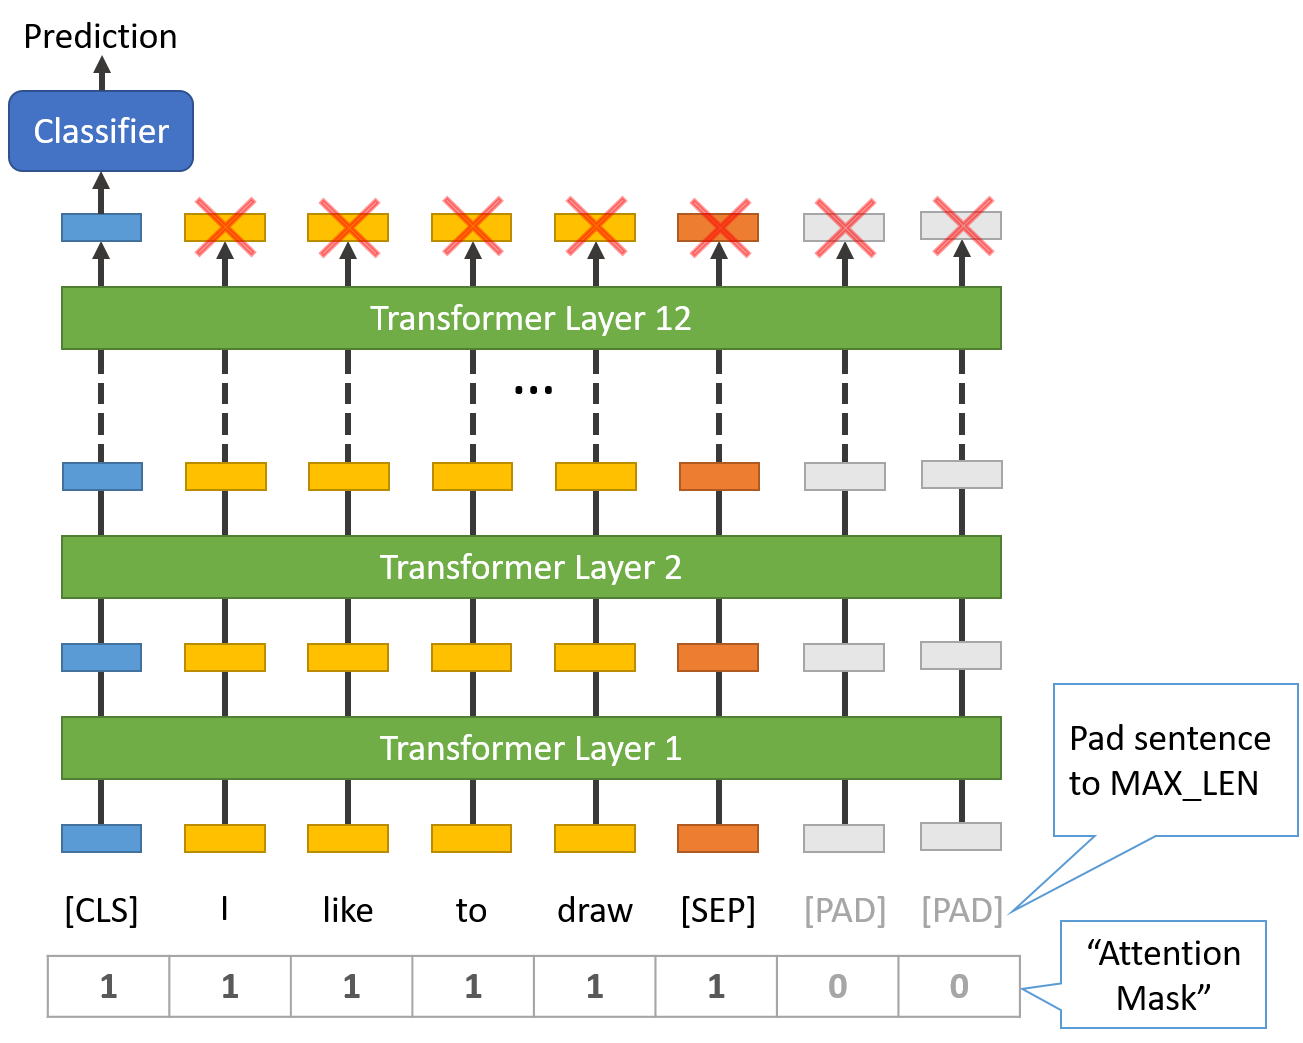
\includegraphics[scale=0.5]{figuras/bert-as-architecture.png}
    % \caption[Así aparece el rótulo en el índice]{Así aparece el rótulo en el texto.}
    \caption[Análisis de Sentimiento - Arquitectura de la solución]{\textbf{Adecuación de la arquitectura de BERT para la solución de problemas de clasificación basados en una frase de entrada. Fuente: \cite{chris_mccormick_and_nick_ryan_bert_2019}}}
    \label{fig-bert-as-architecture}
\end{figure}

%%%%%%%%%%%%%%%%%%%%%%%%%%%%%%%%%%%%%%%%%%%%%%%%%%%%%%%%%%%%%%%%%%%%%%%%%%%%%%%%%%%%%%%%%%%%%%%%%%%%%%%%%%%%%%%

\subsection{Preparación de los datos}
\label{as-preparacion-de-los-datos}

Durante el proceso de preparación de los datos se abordaron dos etapas. La primera de ellas de exploración y saneamiento de los datos. Durante esta primera etapa:

\begin{itemize}
    \item Se identificó y valido que tal como indica la documentación \cite{maas-EtAl:2011:ACL-HLT2011}, el dataset está compuesto por 50000 registros bien balanceados (25000 datos etiquetados como positivos y 25000 datos etiquetados como negativos) como se pudo confirmar una vez fueron cargados los datos. 
    \item Se pudo notar que ciertos registros se encontraban duplicados. Estos registros duplicados fueron removidos.
    \item Se creó y aplicó una función de limpieza que permite para cada una de las reseñas limpiar algunos elementos que podrían causar ruido y carecen de valor en el análisis y entrenamiento del modelo como las etiquetas \acrshort{acr_html}, texto entre corchetes y algunos signos de puntuación.
\end{itemize}

La segunda etapa se basó en un proceso de normalización de los datos de entrada para BERT. Al tratarse BERT de un modelo preentrenado, este espera que los datos de entrada tengan un formato especifico, tal como se indica en la sección \ref{subsection-bert-finetunning}. La normalización de los datos de entrada se basa en la construcción adecuada de los \textit{embeddings} para que el modelo pueda entender cada una de las sentencias de entrada, esto consiste en:

\begin{enumerate}
    \item Como se describe en la arquitectura de la solución (ver figura \ref{fig-bert-as-architecture}), el modelo de BERT tiene dos restricciones:
    \begin{enumerate}
    \item Todas las sentencias de entrada deben tener la misma longitud, por ese motivo las sentencias son truncadas o rellenadas con un token especial denominado [PAD]
    \item La longitud máxima de la sentencia de entrada es de 512 tokens.
    \end{enumerate}
    Al tener sentencias de entrada de longitud variable se optó en este caso por truncar los datos de entrada a una longitud máxima de 512 tokens. En otras palabras estamos basando el entrenamiento en los primeros 512 tokens de cada reseña, desechando el resto de la información. 
    \item Añadir sentencias de entrada que tengan agregados los tokens especiales al comienzo y al final de cada sentencia.
    \begin{enumerate}
    \item El token [SEP] es un token especial que se utiliza para demarcar el fin de una sentencia o la separación entre dos sentencias. En este caso se utiliza como delimitador final de la única sentencia de entrada.
    \item El token [CLS] se debe anteponer a cada sentencia de entrada. Este token es usado en las tareas de clasificación, pero indistintamente del problema a resolver el modelo BERT siempre espera recibirlo como el comienzo de la entrada. La importancia de este token radica en que actúa como una representación agregada para las atareas de clasificación. La última capa oculta de este token se usa como una representación de la sentencia para la clasificación de secuencias.
    \end{enumerate}
    \item Agregar dos embeddings de información para el modelo:
    Al embedding de tokens producto del tokenizador de BERT (Token IDs), se deben agregar dos \textit{embeddings} adicionales:
    \begin{enumerate}
    \item Mask IDs o máscara de atención que diferencia cuales elementos de la secuencia son tokens y cuales son tokens de relleno o padding. Se trata simplemente una matriz de 1s y 0s que indica qué tokens están rellenando y cuáles no. Esta máscara le dice al mecanismo de auto-atención en BERT que no incorpore estos tokens [PAD] en su interpretación de la sentencia.
    \item Segment IDs usado para distinguir diferentes sentencias. En este caso en el que tenemos una sola sentencia se trata de un vector de 0s.
    \end{enumerate}
\end{enumerate}

Adicionalmente es importante mencionar que existen técnicas y trabajos enfocados en cómo manejar la limitación que presenta BERT en cuanto a la extinción de los tokens de la secuencia de entrada. 

Existen tres enfoques distintos basados en el costo computacional:
\begin{itemize}
    \item \textbf{Bajo costo computacional:} Seleccionar una parte del texto original. Los ejemplos incluyen elegir los primeros n tokens, los últimos n tokens o compilar una nueva instancia de texto a partir del principio y el final de la instancia de texto original.
    \item \textbf{Costo computacional medio a alto:} Usar modelos de Transformers recientes (como Longformer) que tienen un límite de 4096 tokens en lugar de 512. Estos nuevos métodos tienen mecanismos de atención modificados que reducen el costo computacional.
    \item \textbf{Alto costo computacional:} Dividir la instancia de texto en fragmentos que se ajusten a un modelo como BERT con un límite estándar de 512 tokens por instancia e implementar el modelo en cada parte por separado, luego unir las representaciones vectoriales resultantes.
\end{itemize}

En el artículo de \cite{Fiok_2021_TextGuideLong} además de proponer un nuevo método llamado Text Guide, que es un método de bajo coste computacional el cual pretende hacer un truncamiento mas inteligente de la instancia de entrada.

Por último mencionar que \cite{FTBERTCLAS_https://doi.org/10.48550/arxiv.1905.05583} en su \textit{paper} hace una comparación usando distintas técnicas para truncar el texto, tomando en algunos casos el principio, en otros casos el final y en algunos casos haciendo combinaciones de distintos segmentos del texto. De este trabajo igual podemos concluir que la diferencia del performance del modelo no es significativa entre las distintas técnicas. 

Por las razones antes expuestas y entendiendo que el m´todo elegido no impactará mucho el performance del modelo,  para este trabajo se decidió utilizar un truncamiento simple tomando los primeros 512 tokens de la sentencia de entrada.


%%%%%%%%%%%%%%%%%%%%%%%%%%%%%%%%%%%%%%%%%%%%%%%%%%%%%%%%%%%%%%%%%%%%%%%%%%%%%%%%%%%%%%%%%%%%%%%%%%%%%%%%%%%%%%%

\subsection{Modelo y Fine Tuning}
\label{as-finetunning}

El modelo de BERT se obtuvo desde Tensorflow Hub (\url{https://www.tensorflow.org/hub}). TensorFlow Hub es un repositorio de modelos de aprendizaje automático preentrenados, listos para poder implementar un fine-tunning.

Se usó como modelo BERT preentrenado la versión bert\_multi\_cased\_L-12\_H-768\_A-12. Para hacer el clasificador se optó por usar el API Keras de Tensorflow tomando las salidas del modelo de BERT, específicamente el pooled\_output (embedding del token [CLS]) y creando una capa única para la tarea de clasificación, para ayudar a prevenir el sobreajuste se hizo un droput de 10\%. En esta última capa, se aplica la función softmax para obtener las probabilidades predichas del modelo entrenado.

Para entrenar el modelo propuesto se utilizo como valores de los hiperparámetros los recomendados en el \textit{paper} de BERT. Según los autores del \textit{paper} BERT no necesita muchas epocas para ser entrenado y recomiendan que sean entre 2 y 4. \cite{https://doi.org/10.48550/arxiv.1810.04805}:

\begin{itemize}
    \item Tamaño del lote = 8
    \item Tasa de aprendizaje = 2e-5
    \item Longitud máxima de secuencia = 512
    \item Épocas = 3
\end{itemize}

\begin{figure}[ht!]
    \centering
    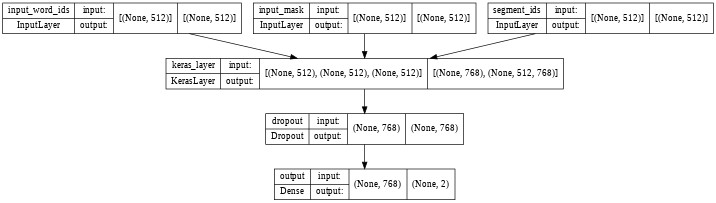
\includegraphics[scale=0.6]{figuras/as-modelo.png}
    % \caption[Así aparece el rótulo en el índice]{Así aparece el rótulo en el texto.}
    \caption[Análisis de Sentimiento - Modelo de la solución]{\textbf{Modelo de BERT propuesto para la solución de este problema de clasificación. En el modelo se observan como entrada las tres embeddings que la conforman, el token embedding, el de segmentación y el posicional, estos van directamente a la capa preentrenada de BERT, luego se agrega una capa de dropout y una última capa que recibe el dropout del embedding del token [CLS] y como salida tiene solo dos neuronas, una para cada clase a predecir. Fuente: Imagen propia}}
    \label{fig-as-modelo}
\end{figure}

El entrenamiento se realizó usando Google Colab y utilizando la GPU (Graphic Processing Unit). La duración del entrenamiento ha sido:

\begin{itemize}
    \item Primera Época = 3368 segundos.
    \item Segunda Época = 3373 segundos. 
    \item Tercera Época = 3372 segundos.
    \item Entrenamiento total = 10113 segundos, aproximadamente 2 horas y 50 minutos.
\end{itemize}

El código fuente del entrenamiento se encuentra en el repositorio Github \url{https://github.com/lsizaguirre/09MIAR-TFM}

%%%%%%%%%%%%%%%%%%%%%%%%%%%%%%%%%%%%%%%%%%%%%%%%%%%%%%%%%%%%%%%%%%%%%%%%%%%%%%%%%%%%%%%%%%%%%%%%%%%%%%%%%%%%%%%

\subsection{Resultados y Conclusiones.}
\label{as-resultados-y-conclusiones}

Podemos observar que con una configuración de red muy sencilla y con los parámetros recomendados para el fine-tunning se obtienen resultados bastante buenos y cercanos a los que definen el estado del arte. Se podría intentar hacer un ajuste más sofisticado y con ello obtener mejores resultados.

Las siguientes imágenes muestran algunas de las métricas obtenidas durante la evaluación del experimento.

\begin{figure}[ht!]
    \centering
    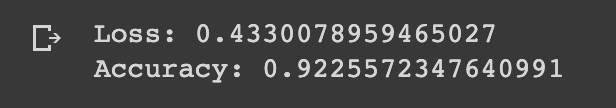
\includegraphics[scale=0.6]{figuras/as-resultados-1.png}
    % \caption[Así aparece el rótulo en el índice]{Así aparece el rótulo en el texto.}
    \caption[Análisis de Sentimiento - Resultados - Accuracy y Loss]{\textbf{Accuracy y Loss obtenidos con el modelo. Fuente: Imagen propia}}
    \label{fig-as-resultados-1}
\end{figure}

\begin{figure}[ht!]
    \centering
    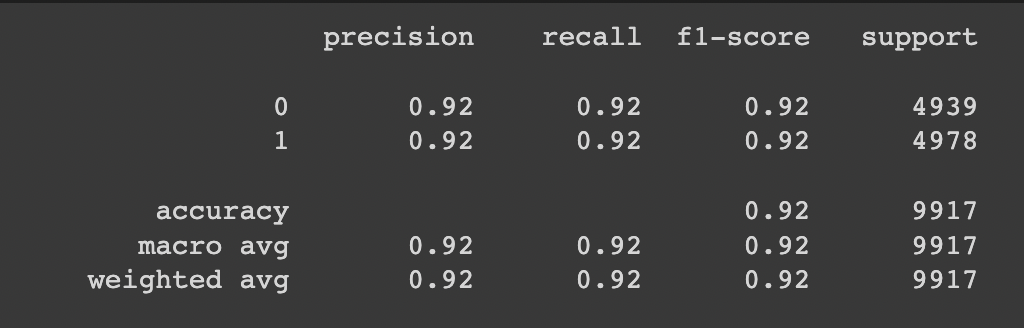
\includegraphics[scale=0.6]{figuras/as-resultados-2.png}
    % \caption[Así aparece el rótulo en el índice]{Así aparece el rótulo en el texto.}
    \caption[Análisis de Sentimiento - Resultados - Métricas de clasificación]{\textbf{Métricas de clasificación obtenidas en el modelo. Fuente: Imagen propia}}
    \label{fig-as-resultados-2}
\end{figure}

\begin{figure}[ht!]
    \centering
    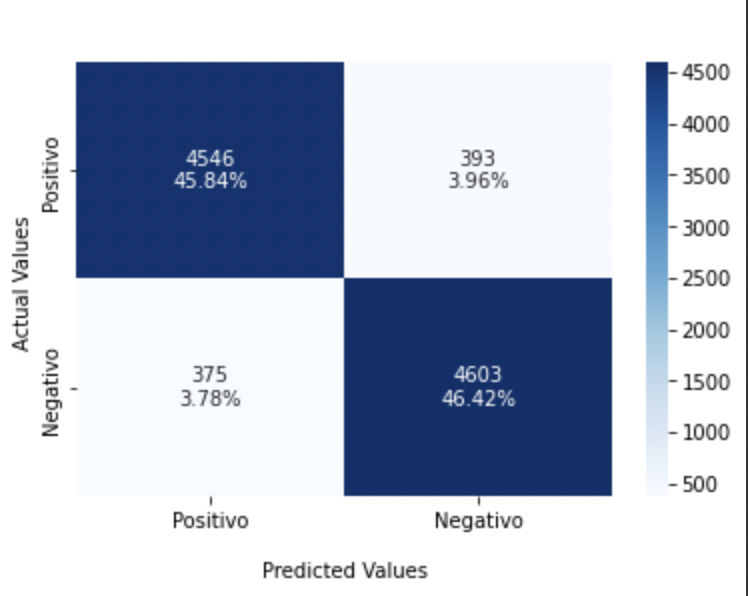
\includegraphics[scale=0.6]{figuras/as-resultados-3.png}
    % \caption[Así aparece el rótulo en el índice]{Así aparece el rótulo en el texto.}
    \caption[Análisis de Sentimiento - Resultados - Matriz de confusión]{\textbf{Matriz de confusión resultado de la evaluación del modelo. Fuente: Imagen propia}}
    \label{fig-as-resultados-3}
\end{figure}


\clearpage 
%%%%%%%%%%%%%%%%%%%%%%%%%%%%%%%%%%%%
% SECTION - PREGUNTAS Y RESPUESTAS 
%%%%%%%%%%%%%%%%%%%%%%%%%%%%%%%%%%%%

\section{Problema de Respuesta a Preguntas}
\label{section-preguntas-y-respuestas}

%%%%%%%%%%%%%%%%%%%%%%%%%%%%%%%%%%%%%%%%%%%%%%%%%%%%%%%%%%%%%%%%%%%%%%%%%%%%%%%%%%%%%%%%%%%%%%%%%%%%%%%%%%%%%%%

\subsection{Descripción del problema}
\label{subsection-qa-descripcion-problema}

Vivimos en una época donde la actividad digital forma parte de nuestro día a día. Todos los días generamos una cantidad enorme de datos e información, interactuando a través de redes sociales, trabajando conectados a Internet, etc. A medida que aumenta la información, se vuelve más difícil recuperar una pieza de información relevante de manera eficiente. En este sentido, la tarea de Respuesta a Preguntas o \textit{Question Answering} (QA, por sus siglas en inglés) es un campo de la ciencia de la computación y el NLP que tiene como objetivo crear sistemas que puedan responder de forma automática preguntas en lenguaje natural.  

Los sistemas QA intentan encontrar automáticamente la respuesta contextual y semánticamente correcta para una pregunta proporcionada en un texto. En general, los tres componentes asociados con los sistemas QA son:

\begin{enumerate}
    \item Clasificación de preguntas
    \item Recuperación de información
    \item Extracción/generación de respuestas
\end{enumerate}

En este trabajo se usará BERT como modelo base para resolver este problema. La idea en este caso es que se le dará un párrafo al modelo de BERT que contendrá información acerca de un tema, y vamos a buscar respuestas con respecto a preguntas relacionadas con ese tema. Para ello, se generarán preguntas cuyas respuestas se encuentren dentro de los textos del párrafo.

%%%%%%%%%%%%%%%%%%%%%%%%%%%%%%%%%%%%%%%%%%%%%%%%%%%%%%%%%%%%%%%%%%%%%%%%%%%%%%%%%%%%%%%%%%%%%%%%%%%%%%%%%%%%%%%

\subsection{Selección del Dataset}
\label{subsection-qa-dataset-imdb}

Para este experimento se usó \textbf{\acrfull{acr_squad}}. Este es un conjunto de datos de respuesta a preguntas publicado en el año 2016 por investigadores de la Universidad de Stanford, junto al \textit{paper} ``\textit{SQuAD: 100000+ Questions for Machine Comprehension of Text}'' \citep{SQUADv1_https://doi.org/10.48550/arxiv.1606.05250}

Existe una segunda versión de SQuAD (v2.0) publicada por los mismos investigadores en el año 2018 en el \textit{paper} ``\textit{Know What You Don't Know: Unanswerable Questions for SQuAD}'' \citep{SQUADv2_https://doi.org/10.48550/arxiv.1806.03822}. Esta versión se diferencia de la primera en que en algunas oportunidades la respuesta no se encuentra en el texto original y está enfocada a ser utilizada en soluciones donde el modelo debe fabricar la respuesta de algún modo. Por simplicidad en este trabajó se utilizó la versión 1.1 de este conjunto de datos.

Este conjunto de datos contiene un total de 107785 preguntas extraídas de un conjunto de 536 artículos seleccionados de la Wikipedia, en un amplio rango de tópicos. Los autores del \textit{paper} mencionan que este conjunto de datos se diferencia a los que se habían publicado con anterioridad en que las respuestas son de formato libre y no están acotadas a un conjunto de opciones lo que hace el problema más interpretativo y con una cantidad bastante grande de opciones. 

Otro aspecto relevante es que los archivos que componen este conjunto de datos se encuentran en \textit{formato .json} y vienen en las siguientes particiones, generadas aleatoriamente:

\begin{itemize}
    \item \textbf{train-v1.1.json:} Es un \gls{gls_json} que contiene el 80\% de los datos y contiene el conjunto de entrenamiento o training set. Es el subconjunto del dataset donde están almacenadas las secuencias que se utilizarán para hacer el entrenamiento.
    \item \textbf{dev-v1.1.json:} Es un \gls{gls_json} que contiene el 10\% de los datos y contiene el conjunto de validación o validation test. Es el subconjunto de datos que se utilizarán para hacer la evaluación.
    \item El 10\% restante de registros son usados para la validación final usada en el benchmark y este conjunto de datos no lo hacen disponible. testing set.
\end{itemize}

%%%%%%%%%%%%%%%%%%%%%%%%%%%%%%%%%%%%%%%%%%%%%%%%%%%%%%%%%%%%%%%%%%%%%%%%%%%%%%%%%%%%%%%%%%%%%%%%%%%%%%%%%%%%%%%

\subsection{Estado del arte}
\label{subsection-qa-estado-del-arte}

Hay dos métricas dominantes utilizadas por muchos conjuntos de datos de respuesta a preguntas, incluido SQuAD: la coincidencia exacta (EM) y puntaje F1. Estos puntajes se calculan en pares individuales de pregunta y respuesta. Cuando son posibles varias respuestas correctas para una pregunta determinada, se calcula la puntuación máxima sobre todas las posibles respuestas correctas. Las puntuaciones generales de EM y F1 se calculan para un modelo promediando las puntuaciones de los ejemplos individuales.

\begin{itemize}
    \item \textbf{Coincidencia exacta o Exact Match (EM, por sus siglas en inglés):} esta métrica es tan simple como parece. Para cada par de pregunta y respuesta, si los caracteres de la predicción del modelo coinciden exactamente con los caracteres de (una de) las respuestas verdaderas, EM = 1; de lo contrario, EM = 0. Esta es una métrica estricta de todo o nada, estar equivocado por un solo carácter da como resultado una puntuación de 0. Al evaluar contra un ejemplo negativo, si el modelo predice cualquier texto, automáticamente recibe un 0 para ese ejemplo.
    \item \textbf{La puntuación F1 o F1 score (en inglés):} es una métrica común para los problemas de clasificación y se usa ampliamente en la tarea de QA. Es apropiado cuando nos preocupamos por igual por la precisión y la memoria. En este caso, se calcula sobre las palabras individuales de la predicción frente a las de la respuesta verdadera. La cantidad de palabras compartidas entre la predicción y la verdad es la base de la puntuación F1: la precisión es la relación entre la cantidad de palabras compartidas y la cantidad total de palabras en la predicción, y el recuerdo o memoria es la relación entre la cantidad de palabras compartidas. al número total de palabras en la verdad fundamental.
\end{itemize}

Es indudable que BERT ha provocado un avance considerable en el estado del arte de varias tareas de NLP. Específicamente en la tarea de QA podemos ver tanto en el leaderboard  de SQuAD como en el de otros conjuntos de datos similares como CoQA \citep{CoQA_https://doi.org/10.48550/arxiv.1808.07042} que la mayoría de modelos que lideran están basados en BERT.

\begin{figure}[ht!]
    \centering
    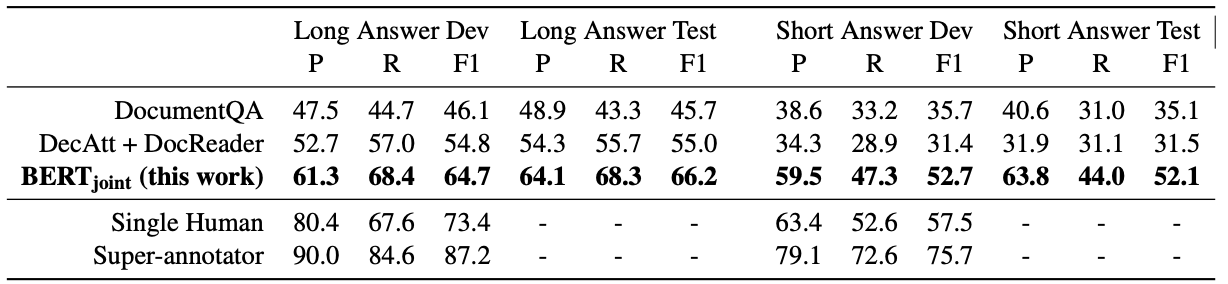
\includegraphics[scale=0.69]{figuras/qa-eda-vshuman.png}
    % \caption[Así aparece el rótulo en el índice]{Así aparece el rótulo en el texto.}
    \caption[Preguntas y Respuestas - Comparación rendimiento BERT vs humanos]{\textbf{En este estudio \cite{BERT_baseline_for_NQ_https://doi.org/10.48550/arxiv.1901.08634} comparan el desempeño de BERT contra un humano común y un humano experto. Se evidencia el mejor desempeño de BERT en ciertos casos. Fuente: \cite{BERT_baseline_for_NQ_https://doi.org/10.48550/arxiv.1901.08634}}}
    \label{fig-qa-eda-vshuman}
\end{figure}

Para evaluar el estado del arte relacionado a la solución de preguntas y respuestas sobre el dataset SQuAD en su versión 1.0 se utilizaron diversas fuentes. 

En el \textit{paper} realizado por \citet{BERT_baseline_for_NQ_https://doi.org/10.48550/arxiv.1901.08634} titulado ``\textit{A BERT Baseline for the Natural Questions}'' los autores concluyen que BERT debe ser la nueva línea base y que constituye un buen punto de partida para los modelos de preguntas y respuestas y \textit{datasets} con características similares. En este mismo estudio los autores comparan el desempeño de BERT con otros modelos que resolvían la tarea en ese momento y además lo compararon con el desempeño de la tarea realizada por un humano común y un humano experto. (ver figura \ref{fig-qa-eda-vshuman}). Los autores concluyen que los resultados obtenidos por los modelos de respuesta a preguntas basados en BERT también se están acercando rápidamente al rendimiento humano informado para estos conjuntos de datos.

Existen otros estudios, como el presentado en el \textit{paper} ``\textit{Comparative Study of Machine Learning Models and BERT on SQuAD}'' de \cite{SQuAD_Comparison_https://doi.org/10.48550/arxiv.2005.11313} donde realizan un análisis comparativo del rendimiento de ciertos modelos populares en el aprendizaje automático y el modelo de BERT sobre SQuAD, brindando BERT una mayor precisión que otros modelos.

En el ranking de la página oficial de SQuAD (\url{https://rajpurkar.github.io/SQuAD-explorer/}) podemos observar muchos modelos basados en ALBERT \cite{ALBERT_https://doi.org/10.48550/arxiv.1909.11942}. ALBERT es una versión de BERT mucho más ligera con 12 millones de parámetros en vez de 110 millones como los que contiene BERT. En el \textit{paper} original de ALBERT llamado ``\textit{ALBERT: A Lite BERT for Self-supervised Learning of Language Representations}''  comparan el desempeño de ALBERT con BERT en las tareas de SQuAD obteniendo resultados bastante similares (ver figura \ref{fig-qa-eda-albert})

\begin{figure}[ht!]
    \centering
    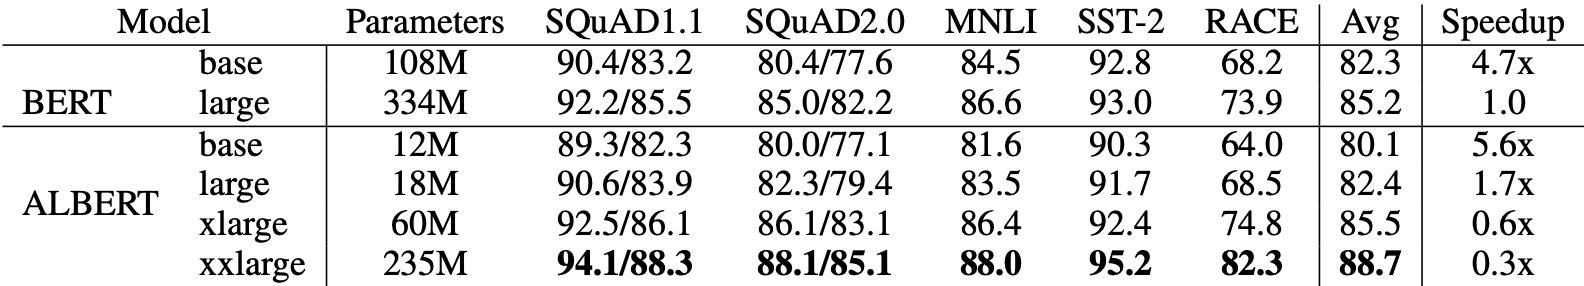
\includegraphics[scale=0.5]{figuras/qa-eda-albert.png}
    % \caption[Así aparece el rótulo en el índice]{Así aparece el rótulo en el texto.}
    \caption[Preguntas y Respuestas - Comparación BERT vs humanos]{\textbf{Comparación de los resultados obtenidos en distintas tareas de NLP entre BERT y su variante ALBERT. Para las tareas SQuAD los dos números equivalen a F1 y EM. Fuente: \cite{ALBERT_https://doi.org/10.48550/arxiv.1909.11942}}}
    \label{fig-qa-eda-albert}
\end{figure}

%%%%%%%%%%%%%%%%%%%%%%%%%%%%%%%%%%%%%%%%%%%%%%%%%%%%%%%%%%%%%%%%%%%%%%%%%%%%%%%%%%%%%%%%%%%%%%%%%%%%%%%%%%%%%%%

\subsection{Arquitectura de la solución}
\label{subsection-qa-arquitectura-de-la-solucion}

Como ya se mencionó en la sección \ref{subsection-arquitectura-bert}, la arquitectura de BERT ha sido diseñada para adaptarse a la resolución de distintos problemas a través de un leve ajuste, por este motivo es que en BERT tenemos dos formas diferentes de manejar la entrada y la salida del modelo. 

Con respecto a la entrada, una de las formas es cuando se tiene un vector que se supone representa toda una frase en su completitud y es básicamente la forma que se utiliza en las tareas de clasificación. La segunda forma de entrada es una lista de vectores, cada uno de los cuales es una representación de las palabras en el contexto que las rodea. Esta segunda forma de entrada es particularmente la que se utiliza en este tipo de problemas al no tratarse de un problema de clasificación como en el experimento anterior.

Como entrada se definieron dos frases, la primera frase representa el texto en el que hay que buscar la información. La segunda frase representa la pregunta que se quiere resolver. En la primera frase, lo que se necesita es buscar dónde empieza y dónde termina la hipotética respuesta a nivel de tokens y ese nivel de tokens luego es traducido a nivel de palabras. De esa forma se busca la respuesta dentro de la primera oración.

Con respecto a la salida, para este caso no se usa el \textit{Pooled Output}, el cual es una representación del token de clasificación [CLS], un embedding de toda la frase. Por el contrario, se usa el \textit{Sequence Output}, el cual está representado por una lista de vectores (embedding), uno para cada una de las palabras, de esta forma se podrá localizar las más probables de ser la el inicio y el final de la respuesta.

Casi siempre que se utiliza BERT para generar la solución de una tarea, lo único que hay que hacer es añadir una capa densa al final antes de hacer ningún ajuste de los parámetros. Estas capas densas se le aplica a cada uno de los elementos, a cada vector y nos va a dar dos posibles respuestas, dos neuronas en la capa de salida.

La primera nos representará una puntuación de qué tan probable es que esa palabra sea la posición inicial en la que empieza la respuesta y la segunda neurona representará una puntuación de qué tan probable es que esa palabra sea la la que finaliza la respuesta De esa forma, simplemente aplicando una capa densa con dos neuronas a cada vector, a cada representación vectorial de las palabras, obtendremos un puntaje de qué tan susceptible es de ser la palabra que inicia o que finaliza la respuesta a la pregunta que estamos buscando.

Finalmente se debe construir un par de listas de todos los puntajes de qué tan probable es que sean el inicio o el final de la respuesta para cada una de las palabras. Una lista para el inicio y otro para el final. La respuesta será la frase o secuencia de palabras contenidas entre el token que tenga el mayor puntaje o probabilidad de ser el inicio de la respuesta y el token con mayor puntaje de ser el final de la respuesta.

Como el proceso de tokenización de BERT tiende a romper palabras, estas se tendrán que reconstruir correctamente.

\begin{figure}[ht!]
    \centering
    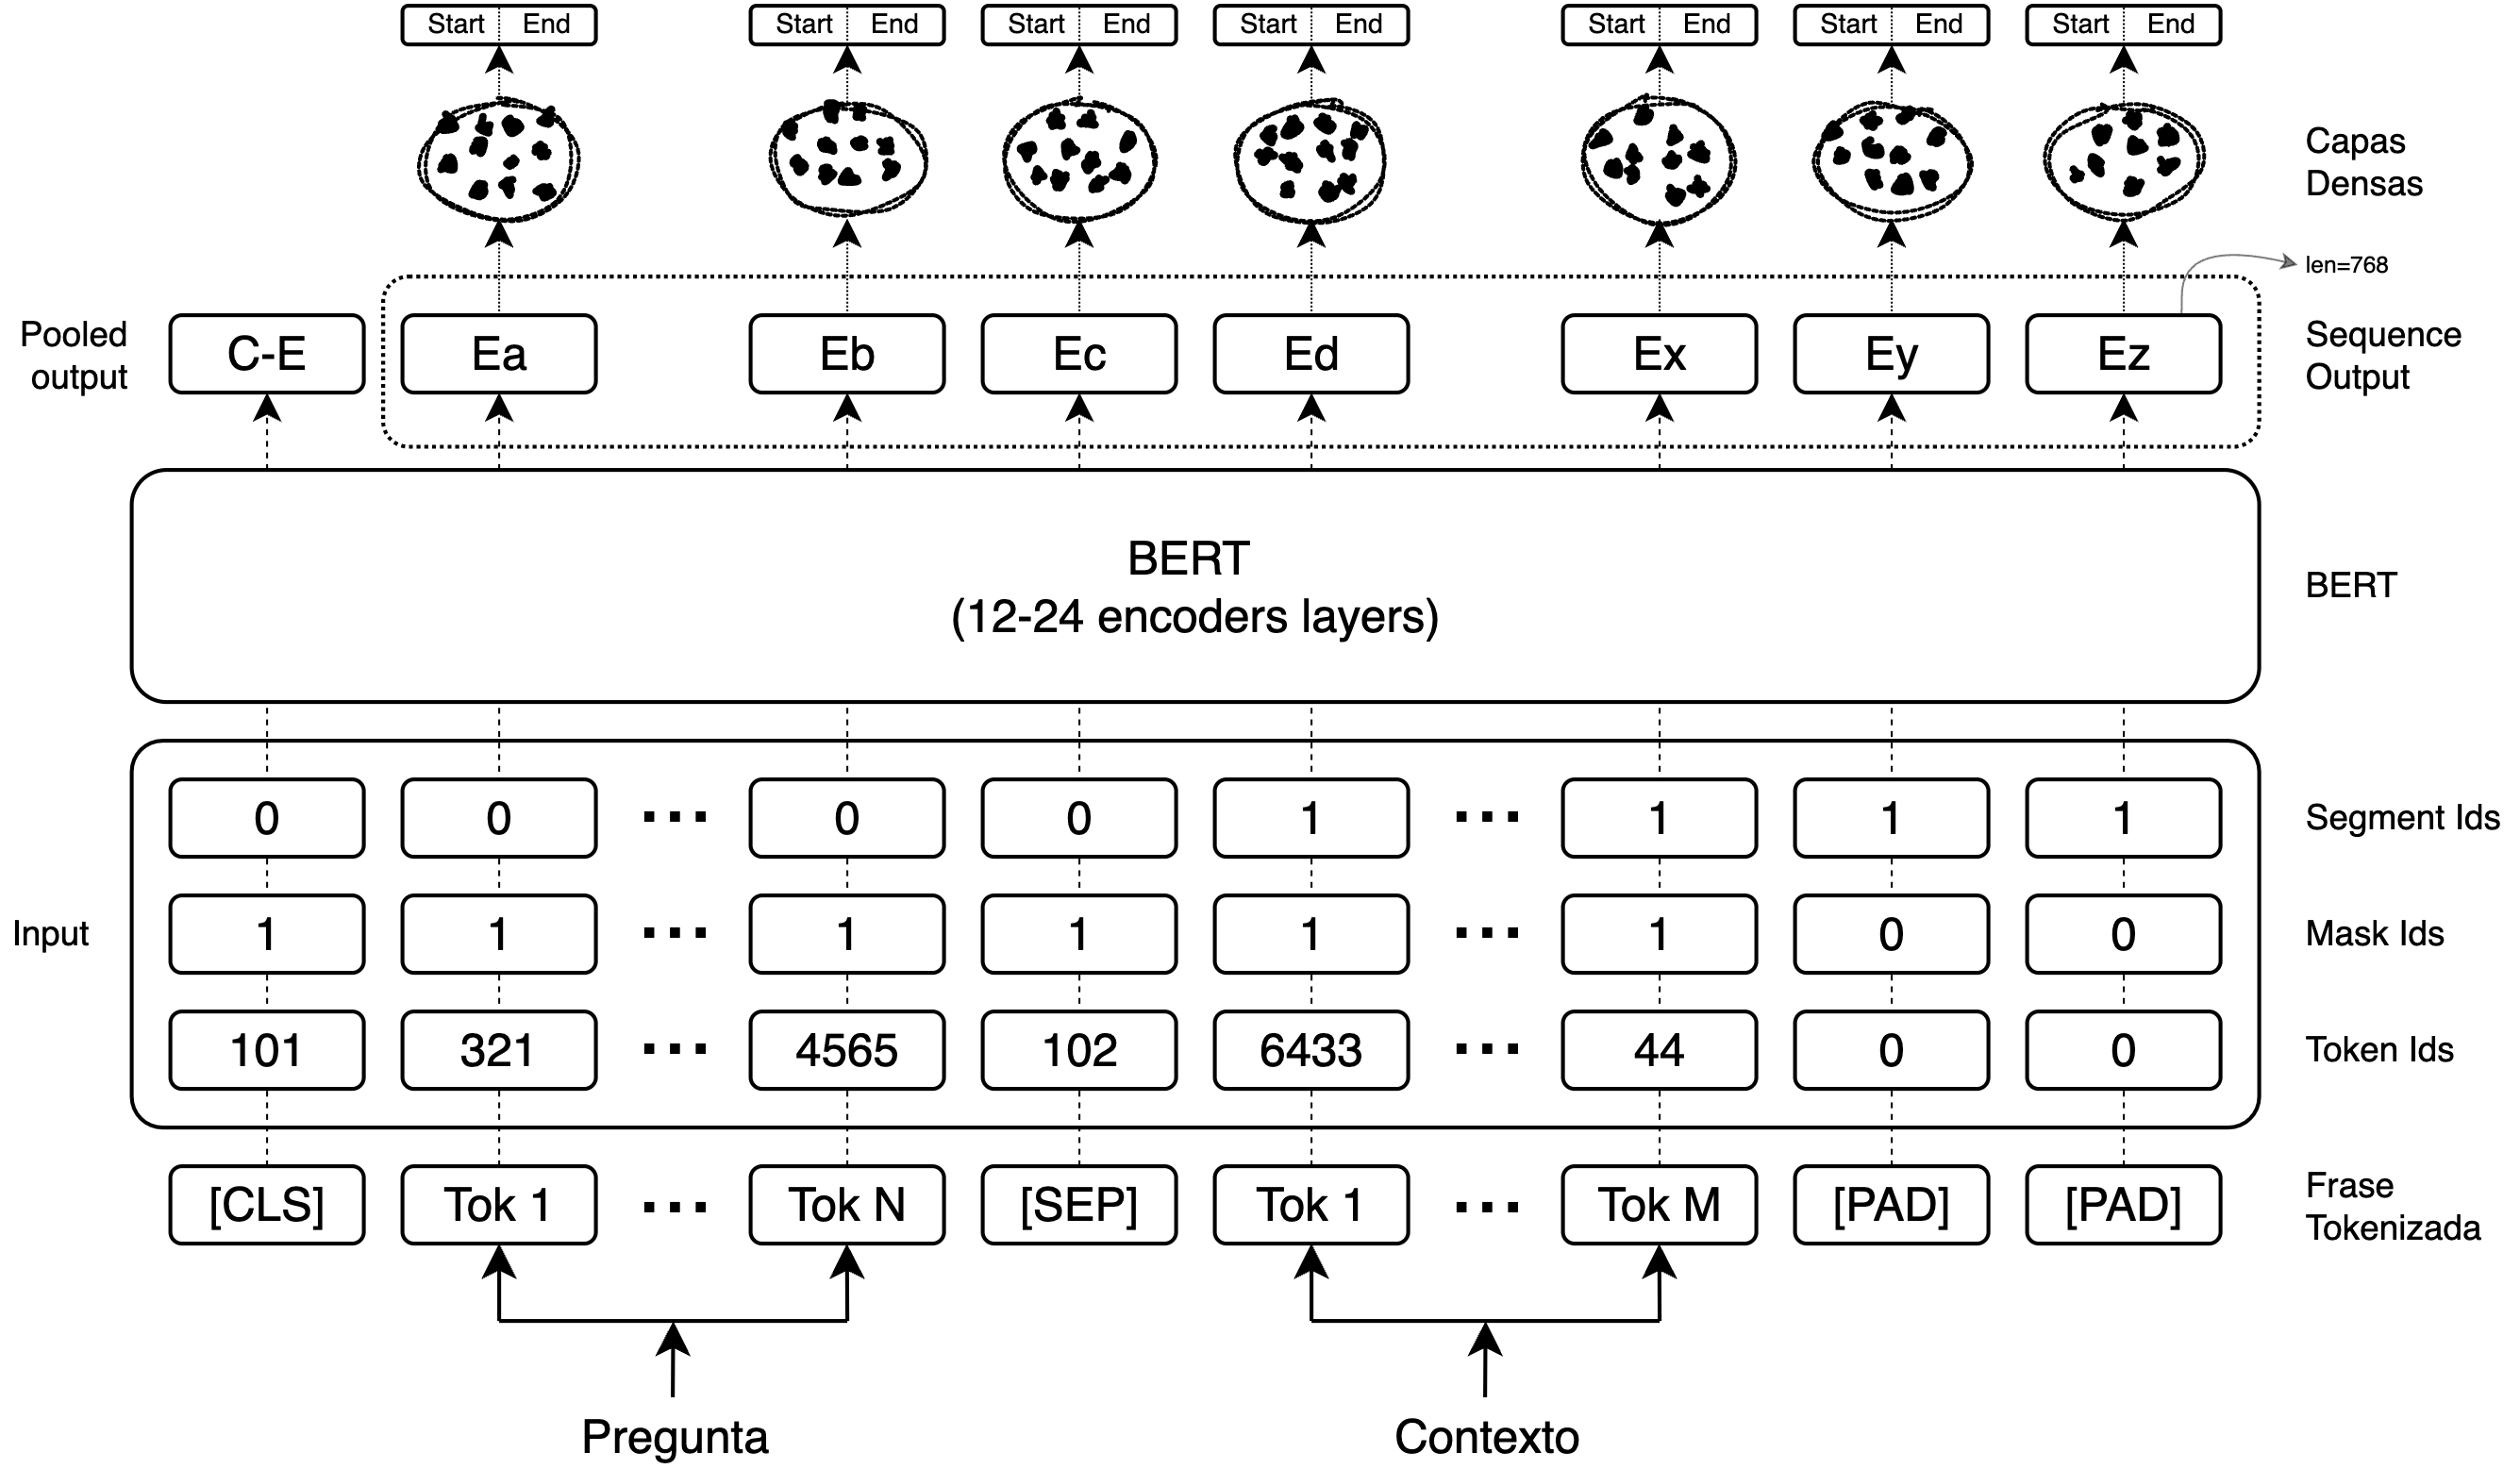
\includegraphics[scale=0.155]{figuras/bert-qa-architecture.png}
    % \caption[Así aparece el rótulo en el índice]{Así aparece el rótulo en el texto.}
    \caption[Preguntas y Respuestas - Arquitectura de la solución]{\textbf{Adecuación de la arquitectura de BERT para la solución de problemas de preguntas y respuestas. Fuente: Imagen propia.}}
    \label{fig-bert-qa-architecture}
\end{figure}

%%%%%%%%%%%%%%%%%%%%%%%%%%%%%%%%%%%%%%%%%%%%%%%%%%%%%%%%%%%%%%%%%%%%%%%%%%%%%%%%%%%%%%%%%%%%%%%%%%%%%%%%%%%%%%%

\subsection{Preparación de los datos}
\label{subsection-qa-preparacion-de-los-datos}

La entrada del modelo BERT para problemas de \textit{question answering} está compuesta por dos frases, la pregunta y el contexto. La forma de manejar la entrada es a través de la estructura mostrada en la figura \ref{fig-bert-qa-architecture}, donde podemos ver:

\begin{enumerate}
    \item Al igual que el experimento anterior y en todos los problemas donde usemos BERT, el token [CLS] se debe anteponer a cada sentencia de entrada. Este token es usado en las tareas de clasificación, pero indistintamente del problema a resolver el modelo BERT siempre espera recibirlo como el comienzo de la entrada.
    \item Seguido al token [CLS] se colocarán los tokens correspondientes a las palabras que componen la pregunta.
    \item A esto le procederá el token especial [SEP] que en este caso tiene un significado distinto dentro de la entrada al experimento anterior. La idea en este caso es que el token [SEP] separará la pregunta del contexto.
    \item En el segment embedding se debe marcar desde el principio de la frase de entrada hasta el token [SEP] como el segmento inicial.
    \item En el resto del token embedding se colocarán los tokens que correspondan al contexto o referencia.
    \item Al igual que en el experimento anterior BERT presenta algunas restricciones con respecto a la entrada:
    \begin{enumerate}
    \item Todas las sentencias de entrada deben tener la misma longitud.
    \item La longitud máxima de la sentencia de entrada es de 384 tokens. Esta longitud es un estándar en el conjunto de datos de SQuAD por dos razones, tener la mayoría de las preguntas y contextos tokenizados sin ningún truncamiento y mantener una longitud limitada para acelerar el entrenamiento.
    \end{enumerate}
\end{enumerate}

A diferencia del problema anterior (ver sección \ref{section-analisis-de-sentimiento}), el conjunto de datos asociado a este problema se encuentra en un \gls{gls_json} que necesita ser preprocesado. Sin embargo, esta tarea de preprocesado de datos es una tarea que se simplifica considerablemente comparado con el proceso del experimento anterior debido a un conjunto de funciones que provee Google para trabajar con el conjunto de datos de SQuAD que ya se encuentran escritas y disponibles en su librería Official.nlp.bert. 

Lo que se logra con estas librerías es transformar los datos de entrenamiento de SQuAD a datos utilizables por las librerías de Tensorflow. Para ello se utilizará la función \textbf{\textit{generate\_tf\_record\_from\_json\_file}}, dejando escrita, su salida, en un
archivo llamado \textbf{\textit{train\_meta\_data}}, divido en cuatro partes. Este archivo ya estará
listo para ser utilizado, también se inicializa el tamaño del batch para el entrenamiento, en este caso será de tamaño 4.

Una vez dado este paso ya se obtienen los datos “tokenizados”, luego a través de la función \textbf{\textit{create\_squad\_dataset}} y a partir de los archivos mencionados con anterioridad, se crea el \textit{dataset} de entrenamiento. De esa forma ya se tendrán listos los datos para entrenar el modelo. 

%%%%%%%%%%%%%%%%%%%%%%%%%%%%%%%%%%%%%%%%%%%%%%%%%%%%%%%%%%%%%%%%%%%%%%%%%%%%%%%%%%%%%%%%%%%%%%%%%%%%%%%%%%%%%%%

\subsection{Modelo y Fine Tuning}
\label{subsection-qa-finetunning}

Al igual que el experimento anterior, el modelo de BERT se obtuvo desde Tensorflow Hub (\url{https://www.tensorflow.org/hub}). Se usó como modelo BERT preentrenado la versión bert\_en\_uncased\_L-12\_H-768\_A-12 al principio se usó la versión bert\_multi\_cased\_L-12\_H-768\_A-12, pensando que se obtendrían mejores resultados usando entradas en distintos idiomas, pero los resultados no fueron buenos. 

Adicionalmente y haciendo uso del API Keras de Tensorflow se creó una ``capa SQuAD'', esta es una capa compuesta por redes neuronales densamente conectadas, la cual será entrenada para devolver dos valores numéricos.

Estos valores representarán dos posiciones en el contexto, que determinarán de dónde se obtendrán el resultado, una vez obtenido el resultado. El resultado calculado se podrá comparar con el resultado esperado y, de esta forma, en base a la evaluación del error cometido, empezar el aprendizaje de las neuronas de la red densamente conectada. 

Como recomienda Tensorflow en su página oficial (\url{https://www.tensorflow.org/text/tutorials/fine_tune_bert}), la función de perdida se implementó a través del método \textbf{\textit{sparse\_categorical\_crossentropy}} de \textbf{\textit{tf.keras.backend}}.

Para entrenar el modelo propuesto se utilizó como valores de los hiperparámetros los recomendados en el \textit{paper} de BERT. Según los autores del \textit{paper} BERT no necesita muchas épocas para ser entrenado y recomiendan que sean entre 2 y 4. \cite{https://doi.org/10.48550/arxiv.1810.04805}:

\begin{itemize}
    \item Tamaño del entrenamiento = 88641 
    \item Número de lotes = 3000 
    \item Tamaño del lote = 4
    \item Tasa de aprendizaje = 2e-5
    \item Longitud máxima de secuencia = 512
    \item Épocas = 3
\end{itemize}

El entrenamiento se realizó usando Google Colab y utilizando la \acrlong{acr_tpu} (\acrshort{acr_tpu}, por sus siglas en inglés). La duración del entrenamiento ha sido:

\begin{itemize}
    \item Primera Época = 12863 segundos.
    \item Segunda Época = 10381 segundos. 
    \item Tercera Época = 11303 segundos.
    \item Entrenamiento total = 34537 segundos, aproximadamente 9 horas y 40 minutos.
\end{itemize}

El código fuente del entrenamiento se encuentra en el repositorio Github \url{https://github.com/lsizaguirre/09MIAR-TFM}

%%%%%%%%%%%%%%%%%%%%%%%%%%%%%%%%%%%%%%%%%%%%%%%%%%%%%%%%%%%%%%%%%%%%%%%%%%%%%%%%%%%%%%%%%%%%%%%%%%%%%%%%%%%%%%%

\subsection{Resultados y Conclusiones.}
\label{subsection-qa-resultados-y-conclusiones}

Este experimento es distinto al anterior en cuanto a la fase de evaluación de los resultados debido a que no se puede hacer de forma directa como en el problema de análisis de sentimiento. 

Para evaluar los modelos, primero se obtienen las predicciones haciendo uso también de un conjunto de funciones que Google pone a disposición para tal fin y estas se usan como entrada para un script de evaluación que se encuentra en la página oficial del \textit{dataset} SQuAD (\url{https://rajpurkar.github.io/SQuAD-explorer/}). 

Este \textit{script} de evaluación en \textit{Python} nos permite evaluar las predicciones bajo las mismas condiciones que son aplicadas en el \textit{paper} de SQuAD (como remover los artículos y signos de puntuación de las frases) y obtener las métricas de Exact Match (EM) y el score F1.

En este caso realizamos dos entrenamientos:

\begin{enumerate}
    \item \textbf{Primer entrenamiento:} \\
    Donde se uso como modelo de BERT la versión bert\_multi\_cased\_L-12\_H-768\_A-12, versión base multilenguaje. Con este modelo obtuvimos las siguientes métricas:
    
    \begin{itemize}
        \item Exact Match (EM) = 29,33\%
        \item F1 Score =  41\%
    \end{itemize}
    
    \item \textbf{Segundo entrenamiento:} \\
    Donde se mantuvieron todos los hiperparámetros con los mismos valores pero se entrenó con va versión bert\_en\_uncased\_L-12\_H-768\_A-12 
    
    \begin{itemize}
        \item Exact Match (EM) = 71,34\%
        \item F1 Score =  80,58\%
    \end{itemize}
    
\end{enumerate}

Con respecto a los resultados podemos deducir:

\begin{itemize}
    \item En el primer entrenamiento no se obtuvieron buenos resultados debido a que no seleccionamos el mejor modelo de BERT con respecto a los datos de entrenamiento. Se eligió trabajar con un modelo multilenguaje cuando en los datos de entrenamiento hay solo frases en ingles, además usamos un modelo entrenado con minúsculas y mayúsculas cuando el script de evaluación transforma cada frase a minúscula en el proceso de evaluación.
    \item En el segundo entrenamiento haciendo uso de un modelo adecuado los resultados fueron bastantes satisfactorios, acercándose a los estándares que definen el estado del arte y muy similares a las capacidades humanas.
\end{itemize}
